\chapter{Results}
\section{Ablation Study on Loss Components}
\label{sec:ablation_loss}

To evaluate the contribution of each loss component to the overall model performance, an ablation study was conducted. Four training configurations were compared:
\begin{enumerate}
    \item $\mathcal{L}_{\text{GAN}} + \mathcal{L}_{\text{L1}}$,
    \item $\mathcal{L}_{\text{GAN}} + \mathcal{L}_{\text{L1}} + \mathcal{L}_{\text{SSIM}}$,
    \item $\mathcal{L}_{\text{GAN}} + \mathcal{L}_{\text{L1}} + \mathcal{L}_{\text{LPIPS}}$, and
    \item the full combination $\mathcal{L}_{\text{GAN}} + \mathcal{L}_{\text{L1}} + \mathcal{L}_{\text{SSIM}} + \mathcal{L}_{\text{LPIPS}}$.
\end{enumerate}
This analysis aimed to isolate the contribution of each additional loss term to both quantitative performance and visual reconstruction quality. The evaluation was conducted using the same IQA metrics employed throughout the thesis, namely SSIM, PSNR, LPIPS, SAM, MAE, and RMSE. Several training loops were conducted using the same preprocessing procedure described in Section~\ref{subsec:preprocessing}. All models were trained under identical settings, hyperparameters, datasets, and number of epochs to ensure a fair and consistent comparison across the different loss configurations.

Table~\ref{tab:ablation_quantitative} summarizes the quantitative performance across the four loss configurations. As shown, the baseline configuration without SSIM and LPIPS achieved the lowest performance across most metrics, with the exception of PSNR. This configuration also represents the weakest setup in terms of overall image quality. As illustrated in Figure~\ref{fig:ablation_samples}(b), images generated by the baseline model differ significantly from the ground truth, both texturally and perceptually. 

\begin{table}[h!]
    \centering
    \resizebox{\textwidth}{!}{%
        \begin{tabular}{lcccccc}
            \toprule
            \textbf{Loss Configuration}                                                                                   & \textbf{SSIM $\uparrow$} & \textbf{PSNR (dB) $\uparrow$} & \textbf{LPIPS $\downarrow$} & \textbf{SAM~(°) $\downarrow$} & \textbf{MAE $\downarrow$} & \textbf{RMSE $\downarrow$} \\
            \midrule
            $\mathcal{L}_{\text{GAN}} + \mathcal{L}_{\text{L1}}$                                                          & 0.820                    & 26.38                         & 0.287                       & 6.47                          & 229                       & 441                        \\
            $\mathcal{L}_{\text{GAN}} + \mathcal{L}_{\text{L1}} + \mathcal{L}_{\text{SSIM}}$                              & \textbf{0.862}           & \textbf{27.67}                & 0.399                       & \textbf{5.43}                 & 198                       & \textbf{380}               \\
            $\mathcal{L}_{\text{GAN}} + \mathcal{L}_{\text{L1}} + \mathcal{L}_{\text{LPIPS}}$                             & 0.842                    & 27.58                         & \textbf{0.213}              & 5.73                          & 201                       & 385                        \\
            $\mathcal{L}_{\text{GAN}} + \mathcal{L}_{\text{L1}} + \mathcal{L}_{\text{SSIM}} + \mathcal{L}_{\text{LPIPS}}$ & 0.859                    & 27.65                         & 0.224                       & 5.44                          & \textbf{195}              & 382                        \\
            \bottomrule
        \end{tabular}%
    }
    \caption{Quantitative results of the ablation study across different loss configurations. Arrows ($\uparrow$ / $\downarrow$) indicate whether higher or lower values denote better performance, respectively.
        Best values per metric are shown in bold.}
    \label{tab:ablation_quantitative}
\end{table}
Notably, integrating SSIM alone yielded the highest quantitative scores in several metrics. However, the qualitative results under this configuration reveal perceptual inconsistencies and reduced visual realism. This discrepancy arises because SSIM does not always align with human perceptual judgments of image similarity. As reported by NVIDIA in~\cite{nvidia_Understanding_SSIM}, SSIM can overemphasize small intensity variations in dark regions, overlook significant color shifts, and assign high similarity near edges even when visible artifacts are present.

\begin{figure}[h!]
    \centering
    \setlength{\tabcolsep}{2pt} % horizontal padding between columns
    \renewcommand{\arraystretch}{1.0} % vertical padding

    % Adjust width so that 6 images fit one row across the text width
    % (tweak 0.155\textwidth to 0.158 or 0.152 if needed)
    \begin{tabular}{*{6}{c}}
        % \toprule
        (a)                                                                      & (b) & (c) & (d) & (e) & (f) \\
        % \midrule

        % ------------------- Row 1 -------------------
        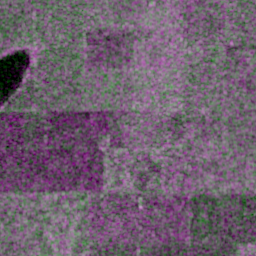
\includegraphics[width=0.155\textwidth]{img/ablation/sample_1/sar.png}   &
        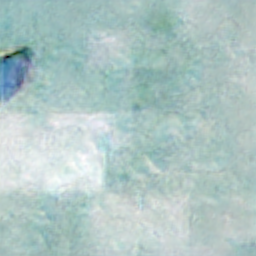
\includegraphics[width=0.155\textwidth]{img/ablation/sample_1/none.png}  &
        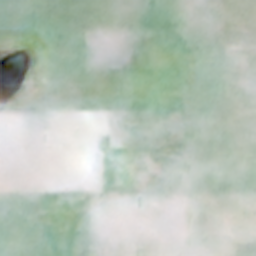
\includegraphics[width=0.155\textwidth]{img/ablation/sample_1/ssim.png}  &
        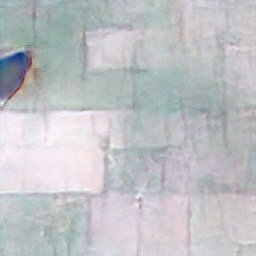
\includegraphics[width=0.155\textwidth]{img/ablation/sample_1/lpips.png} &
        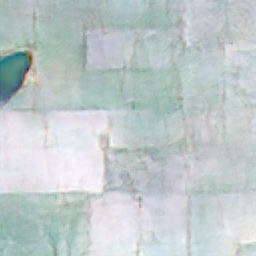
\includegraphics[width=0.155\textwidth]{img/ablation/sample_1/all.png}   &
        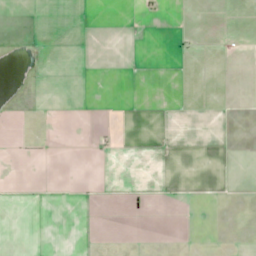
\includegraphics[width=0.155\textwidth]{img/ablation/sample_1/gt.png}                                  \\
        % ------------------- Row 2 -------------------
        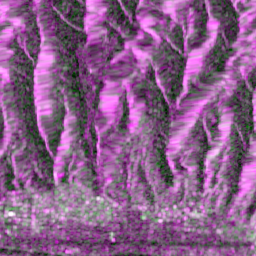
\includegraphics[width=0.155\textwidth]{img/ablation/sample_2/sar.png}   &
        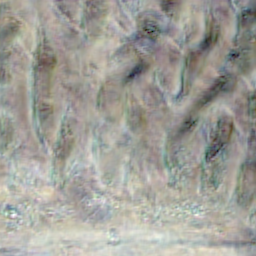
\includegraphics[width=0.155\textwidth]{img/ablation/sample_2/none.png}  &
        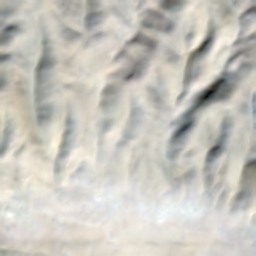
\includegraphics[width=0.155\textwidth]{img/ablation/sample_2/ssim.png}  &
        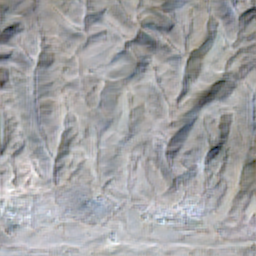
\includegraphics[width=0.155\textwidth]{img/ablation/sample_2/lpips.png} &
        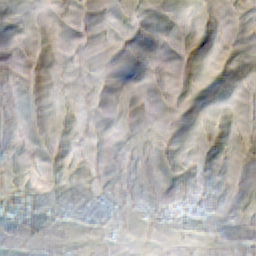
\includegraphics[width=0.155\textwidth]{img/ablation/sample_2/all.png}   &
        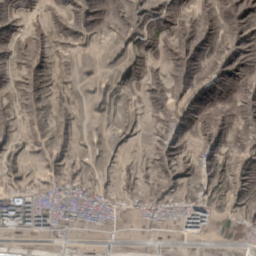
\includegraphics[width=0.155\textwidth]{img/ablation/sample_2/gt.png}                                  \\
        % ------------------- Row 3 -------------------
        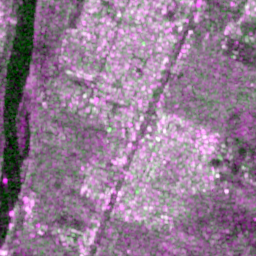
\includegraphics[width=0.155\textwidth]{img/ablation/sample_3/sar.png}   &
        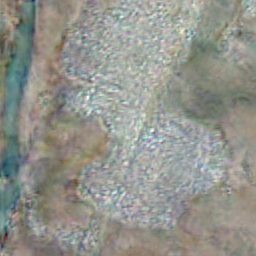
\includegraphics[width=0.155\textwidth]{img/ablation/sample_3/none.png}  &
        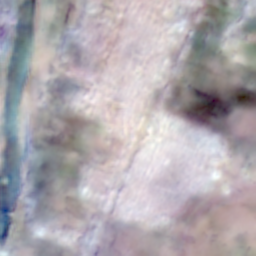
\includegraphics[width=0.155\textwidth]{img/ablation/sample_3/ssim.png}  &
        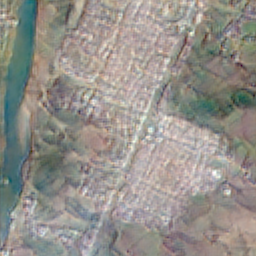
\includegraphics[width=0.155\textwidth]{img/ablation/sample_3/lpips.png} &
        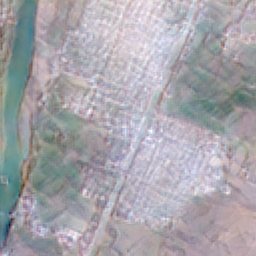
\includegraphics[width=0.155\textwidth]{img/ablation/sample_3/all.png}   &
        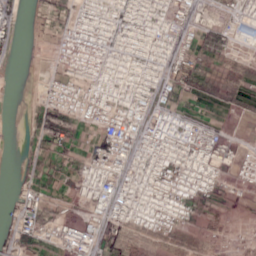
\includegraphics[width=0.155\textwidth]{img/ablation/sample_3/gt.png}                                  \\
        % ------------------- Row 4 -------------------
        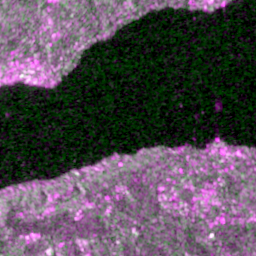
\includegraphics[width=0.155\textwidth]{img/ablation/sample_4/sar.png}   &
        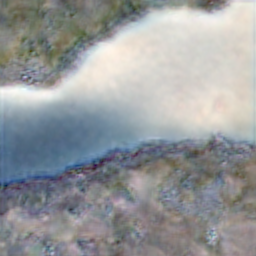
\includegraphics[width=0.155\textwidth]{img/ablation/sample_4/none.png}  &
        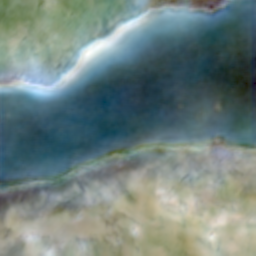
\includegraphics[width=0.155\textwidth]{img/ablation/sample_4/ssim.png}  &
        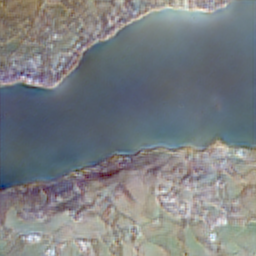
\includegraphics[width=0.155\textwidth]{img/ablation/sample_4/lpips.png} &
        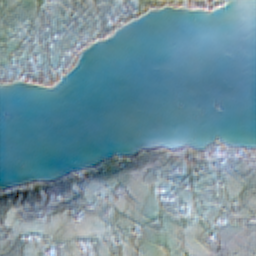
\includegraphics[width=0.155\textwidth]{img/ablation/sample_4/all.png}   &
        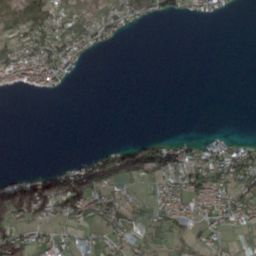
\includegraphics[width=0.155\textwidth]{img/ablation/sample_4/gt.png}                                  \\
        % \bottomrule
    \end{tabular}

    \caption{%
    Qualitative ablation results showing representative samples (rows) under four configurations (columns):\\
    \textbf{(a)}~Input SAR (pseudo RGB)\\
    \textbf{(b)}~$\mathcal{L}_{\text{GAN}}{+}\mathcal{L}_{\text{L1}}$\\
    \textbf{(c)}~$\mathcal{L}_{\text{GAN}}{+}\mathcal{L}_{\text{L1}}{+}\mathcal{L}_{\text{SSIM}}$\\
    \textbf{(d)}~$\mathcal{L}_{\text{GAN}}{+}\mathcal{L}_{\text{L1}}{+}\mathcal{L}_{\text{LPIPS}}$\\
    \textbf{(e)}~all four losses combined\\
    \textbf{(f)}~ground-truth Sentinel-2 optical image (RGB bands).
    }
    \label{fig:ablation_samples}
\end{figure}

Since the primary objective of LPIPS is to measure perceptual similarity, incorporating it into the baseline configuration led to notable improvements in the preservation of low-level features. As illustrated in column~(d) of Figure~\ref{fig:ablation_samples}, the model was able to maintain sharper edges and more distinct boundaries. Moreover, the generated images appear visually more realistic and closely resemble the ground truth in texture and detail. However, the colour reproduction achieved with LPIPS is slightly inferior to that obtained using SSIM, as the SSIM-based model produces more natural and accurate colours overall.

The full combination of all four losses achieved the best balance between pixel-level accuracy, perceptual realism, and structural coherence. 
Its SAM values were the second best, differing only marginally from the SSIM-only configuration. 
By incorporating both SSIM and LPIPS, the model attains an effective balance between color, luminance, and perceptual realism, as shown in column~(e) of Figure~\ref{fig:ablation_samples}. 
Similar findings were also reported by~\cite{s2o_ViT_cGAN} and~\cite{CR_RS_GAN_s2o}. 
 
Overall, the results demonstrate the incremental benefit of incorporating perceptual and structural similarity terms alongside the adversarial $\mathcal{L}_{\text{GAN}}$ and $\mathrm{L1}$ objectives. 
